\chapter{ Modul - Vokabeltrainer Englisch }
\label{has:voc-module}

\section{ Hauptseite }
\label{has:voc-module-mainpage}
\begin{description}
	\item[Titel] \emph{ Hauptseite }
	\item[Textbereich] \texttt{ vocabulary/index.html }
	\item[Übung] keine
	\item[Wo bin ich] \emph{\\Du bist hier:\\Vokabeltrainer - Englisch\\Modul-Hauptseite}
	\item[Navigation] Links zu den ersten Lern- und Übungsseiten
	\begin{description}
		\item[Lernen] \prettyref{has:voc-learn-page0}
		\item[Üben] \prettyref{has:voc-practice-page0}
	\end{description}
	\item[Hilfe] keine
\end{description}

\section{ Statistik }
\label{has:voc-module-stats}
\begin{wrapfigure}{r}{0.45\textwidth}
	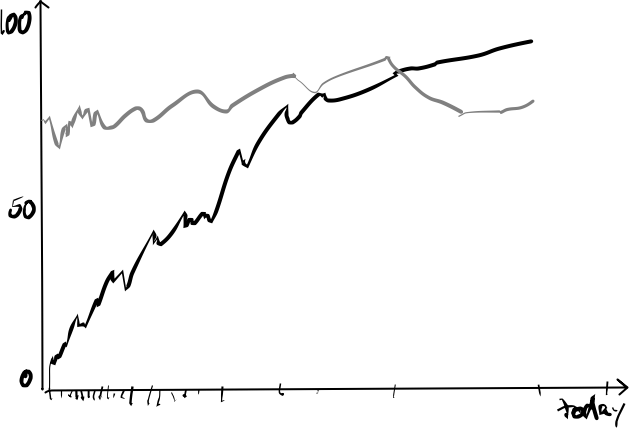
\includegraphics[width=0.4\textwidth]{voc-stats.png}
\end{wrapfigure}
In der Statistik wird ein Prozentsatz-Wert gegen das Datum aufgetragen, dabei wird das Datum logarithmisch im Alter skaliert.

Pauschal wird es zwei Einträge geben:
\begin{description}
	\item[grau] Prozentsatz der richtigen Antworten in der jeweiligen Übung.
	\item[schwarz] Prozentsatz der gelernten Vokabeln im Zusammenhang zum gesamten Wortschatz. Allerdings produziert jeder Wortschatz eine eigene Linie. Dies ist somit eine Art globaler Fortschrittsbalken.
\end{description}


\section{ Lernseiten }
\label{has:voc-learn}

\begin{itemize}
	\item Jede \texttt{Lernseite} ist mit einer \texttt{Übung} verknüpft.
	\item Es gibt keine \texttt{Hilfetexte}.
	\item Jede Lernseite zeigt die Vokabeln der \texttt{Datenbank} alphabetisch an.
	\item Über eine Filter-Einstellung lassen sich optional nur entsprechende Teilmengen anzeigen bzw. schon gelernte Vokabeln ausblenden. \\
		($\{1, 2, \ldots, 5, \text{gar Keine}\}$)
\end{itemize}

\subsection{ Lernen - Hauptseite }
\label{has:voc-learn-page0}
\begin{description}
	\item[Titel] \emph{ Lernen - Hauptseite }
	\item[Textbereich] \texttt{vocabulary/learn/index.html}
	\item[Wo bin ich] \emph{\\Du bist hier:\\Vokabeltrainer - Englisch\\Lernen Hauptseite}
	\item[Hilfe] keine
	\item[Überseite] keine
	\item[Unterseiten] :
	\begin{itemize}
		\item \prettyref{has:voc-learn-page1}
		\item \prettyref{has:voc-learn-page2}
		\item \prettyref{has:voc-learn-page3}
		\item \prettyref{has:voc-learn-page4}
		\item \prettyref{has:voc-learn-page5}
	\end{itemize}
\end{description}


\subsection{ Grundwortschatz }
\label{has:voc-learn-page1}
\begin{description}
	\item[Titel] \emph{ Grundwortschatz }
	\item[Übung] \prettyref{has:voc-practice-page1}
	\item[Datenbank] \texttt{ vocabulary/db/grundwortschatz-de->en.csv }
	\item[Wo bin ich] \emph{\\Du bist hier:\\Vokabeltrainer - Englisch\\Lernen - Grundwortschatz}
	\item[Unterseiten] keine
	\item[Überseite] \prettyref{has:voc-learn-page0}
\end{description}

\subsection{ Aufbauwortschatz }
\label{has:voc-learn-page2}
\begin{description}
	\item[Titel] \emph{ Aufbauwortschatz }
	\item[Lernseite] \prettyref{has:voc-practice-page2}
	\item[Datenbank] \texttt{ vocabulary/db/aufbauwortschatz-de->en.csv }
	\item[Wo bin ich] \emph{\\Du bist hier:\\Vokabeltrainer - Englisch\\Lernen - Aufbauwortschatz}
	\item[Unterseiten] keine
	\item[Überseite] \prettyref{has:voc-learn-page0}
\end{description}

\subsection{ Spezialwortschatz }
\label{has:voc-learn-page3}
\begin{description}
	\item[Titel] \emph{ Spezialwortschatz }
	\item[Lernseite] \prettyref{has:voc-practice-page3}
	\item[Datenbank] \texttt{ vocabulary/db/spezialwortschatz-de->en.csv }
	\item[Wo bin ich] \emph{\\Du bist hier:\\Vokabeltrainer - Englisch\\Lernen - Spezialwortschatz}
	\item[Unterseiten] keine
	\item[Überseite] \prettyref{has:voc-learn-page0}
\end{description}

\subsection{ Umfangreicher Wortschatz }
\label{has:voc-learn-page4}
\begin{description}
	\item[Titel] \emph{ Umfangreicher Wortschatz }
	\item[Lernseite] \prettyref{has:voc-practice-page4}
	\item[Datenbank] \texttt{ vocabulary/db/umfangreicher\_wortschatz-de->en.csv }
	\item[Wo bin ich] \emph{\\Du bist hier:\\Vokabeltrainer - Englisch\\Lernen - Umfangreicher Wortschatz}
	\item[Unterseiten] keine
	\item[Überseite] \prettyref{has:voc-learn-page0}
\end{description}

\subsection{ Umfangreicher Wortschatz zu Wirtschaft und Finanzen }
\label{has:voc-learn-page5}
\begin{description}
	\item[Titel] \emph{ Umfangreicher Wortschatz zu Wirtschaft und Finanzen }
	\item[Lernseite] \prettyref{has:voc-practice-page5}
	\item[Datenbank] \texttt{ vocabulary/db/umfangreicher\_wortschatz\_\\wirtschaft\_finanzen-de->en.csv }
	\item[Wo bin ich] \emph{\\Du bist hier:\\Vokabeltrainer - Englisch\\Lernen - Umfangreicher Wortschatz (Wirtschaft, Finanzen)}
	\item[Unterseiten] keine
	\item[Überseite] \prettyref{has:voc-learn-page0}
\end{description}

\section{ Übungsseiten }
\label{has:voc-practice}

%\subsection{ Aufbau einer Übung }
%\label{has:voc-practice-structure}
\begin{itemize}
	\item Jede Übung ist mit einer \texttt{Lernseite} verknüpft.
	\item Es gibt keine \texttt{Hilfetexte}.
	\item Jede Übung besteht aus einer Reihe von Aufgaben (üblicherweise 20).
	\item Eine Aufgabe besteht aus dem zu übersetzenden Wort und einem Eingabefeld, in dem die gesuchte Übersetzung eingetragen werden muss.
	\item Die zu übersetzenden Vokabeln werden durch die \texttt{Datenbank} definiert.
		Jede Vokabel hat dabei einen internen \texttt{Zähler}, welcher bei richtiger Antwort $+1$ und bei falscher Antwort $=0$ gesetzt wird.
		Für die Aufgaben einer Übung werden jeweils zufällige Variablen mit \texttt{Zähler} $<5$ gewählt (Stichwort: 5-Fächer-Lernen).

\end{itemize}

Die Antwort wird durch eine der Tasten \texttt{TAB} oder \texttt{ENTER} bestätigt. 
Die Antwort wird sofort nach Bestätigung durch das Programm geprüft. 
Neben dem Eingabefeld erscheint ein \emph{richtig} oder \emph{falsch} Icon (\texttt{icons/success.png, icons/fail.png}), ein Zähler wird je nach Korrektheit hochgezählt und bei falscher Antwort erscheint zusätzlich die Musterlösung.
Zeitgleich wird die nächste Aufgabe aufgedeckt, alle bisherigen Aufgaben werde nach oben verschoben und ihr Alpha-Wert wird jeweils um 1/3 herabgesetzt.
So sind jeweils die letzten paar Aufgaben sichtbar.

\subsection{ Üben - Hauptseite }
\label{has:voc-practice-page0}
\begin{description}
	\item[Titel] \emph{ Üben - Hauptseite }
	\item[Textbereich] \texttt{ vocabulary/practice/index.html }
	\item[Wo bin ich] \emph{\\Du bist hier:\\Vokabeltrainer - Englisch\\Üben Hauptseite}
	\item[Hilfe] keine
	\item[Überseite] keine
	\item[Unterseiten] :
	\begin{itemize}
		\item \prettyref{has:voc-practice-page1}
		\item \prettyref{has:voc-practice-page2}
		\item \prettyref{has:voc-practice-page3}
		\item \prettyref{has:voc-practice-page4}
		\item \prettyref{has:voc-practice-page5}
	\end{itemize}
\end{description}

\subsection{ Grundwortschatz }
\label{has:voc-practice-page1}
\begin{description}
	\item[Titel] \emph{ Grundwortschatz }
	\item[Lernseite] \prettyref{has:voc-learn-page1}
	\item[Datenbank] \texttt{ vocabulary/db/grundwortschatz-de->en.csv }
	\item[Wo bin ich] \emph{\\Du bist hier:\\Vokabeltrainer - Englisch\\Üben - Grundwortschatz}
	\item[Unterseiten] keine
	\item[Überseite] \prettyref{has:voc-practice-page0}
\end{description}

\subsection{ Aufbauwortschatz }
\label{has:voc-practice-page2}
\begin{description}
	\item[Titel] \emph{ Aufbauwortschatz }
	\item[Lernseite] \prettyref{has:voc-learn-page2}
	\item[Datenbank] \texttt{ vocabulary/db/aufbauwortschatz-de->en.csv }
	\item[Wo bin ich] \emph{\\Du bist hier:\\Vokabeltrainer - Englisch\\Üben - Aufbauwortschatz}
	\item[Unterseiten] keine
	\item[Überseite] \prettyref{has:voc-practice-page0}
\end{description}

\subsection{ Spezialwortschatz }
\label{has:voc-practice-page3}
\begin{description}
	\item[Titel] \emph{ Spezialwortschatz }
	\item[Lernseite] \prettyref{has:voc-learn-page3}
	\item[Datenbank] \texttt{ vocabulary/db/spezialwortschatz-de->en.csv }
	\item[Wo bin ich] \emph{\\Du bist hier:\\Vokabeltrainer - Englisch\\Üben - Spezialwortschatz}
	\item[Unterseiten] keine
	\item[Überseite] \prettyref{has:voc-practice-page0}
\end{description}

\subsection{ Umfangreicher Wortschatz }
\label{has:voc-practice-page4}
\begin{description}
	\item[Titel] \emph{ Umfangreicher Wortschatz }
	\item[Lernseite] \prettyref{has:voc-learn-page4}
	\item[Datenbank] \texttt{ vocabulary/db/umfangreicher\_wortschatz-de->en.csv }
	\item[Wo bin ich] \emph{\\Du bist hier:\\Vokabeltrainer - Englisch\\Üben - Umfangreicher Wortschatz}
	\item[Unterseiten] keine
	\item[Überseite] \prettyref{has:voc-practice-page0}
\end{description}

\subsection{ Umfangreicher Wortschatz zu Wirtschaft und Finanzen }
\label{has:voc-practice-page5}
\begin{description}
	\item[Titel] \emph{ Umfangreicher Wortschatz zu Wirtschaft und Finanzen }
	\item[Lernseite] \prettyref{has:voc-learn-page5}
	\item[Datenbank] \texttt{ vocabulary/db/umfangreicher\_wortschatz\_\\wirtschaft\_finanzen-de->en.csv }
	\item[Wo bin ich] \emph{\\Du bist hier:\\Vokabeltrainer - Englisch\\Üben - Umfangreicher Wortschatz (Wirtschaft, Finanzen)}
	\item[Unterseiten] keine
	\item[Überseite] \prettyref{has:voc-practice-page0}
\end{description}

